% !TEX root = ../main.tex
\section{Introduction}
\label{sec:intro}

End-to-end driving policies are compared by benchmark scores, and a deployment decision is,
implicitly, a bet that the rank those scores produce will still hold once the policy is driving at
the new site, not just on someone else's roads. Taking that bet blindly is a bad idea: on scenes
where a pedestrian is near the ego corridor, a policy's rank on
nuScenes' open-loop metrics or on NAVSIM's leaderboard score predicts its rank at the deployment site
only about as well as a coin flip ($\rho=-0.54$--$+0.49$; \cref{sec:bench}). The reason is not noise
but mechanism: a score is an outcome measure, and an outcome can be right for the wrong reason. A
policy that never approaches a pedestrian because it plans short trajectories scores as well as one
that sees the pedestrian and yields, and the two behave very differently the first time the scene
changes. Telling them apart means asking \emph{why} the score came out as it did, usually from little
data: a closed-loop simulator for the target domain, or a fleet
test, is exactly what the decision is meant to save.

We propose a \emph{check-up}: a short list of exams, each with a control and a known normal range,
whose results are read as a diagnosis rather than a ranking (\cref{tab:exams}). Every exam is a
counterfactual edit of real frames. We remove the pedestrian from the ego corridor, or re-render the
frame at night, and read the change in the planned trajectory; an independent detector verifies every
edit. The central exam is a \emph{hazard-sensitivity curve}, measuring how much farther the whole
planned trajectory stays from the pedestrian's logged future because the policy can see the
pedestrian, against a model-independent hazard level. A specificity term applies a minimal-change
principle: when no reaction is needed, the plan should not move.

\begin{figure}[t]
\centering
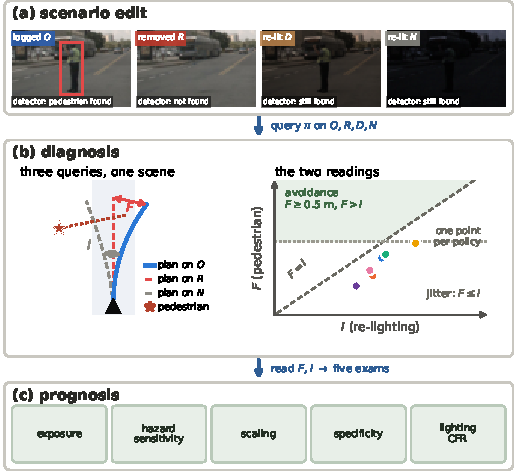
\includegraphics[width=\columnwidth]{figures/frame1c.pdf}
\caption{\textbf{The check-up, on one worked example.} (a)~A logged frame $O$ and its two edits,
pedestrian removed $R$ and re-lit $N$, each checked by a detector no policy shares. (b)~The policy is
queried on all three; joining the plans at equal times gives two numbers, the displacement $F$ the
pedestrian causes and the displacement $I$ the lighting causes, and the right panel places the
policies on those axes. (c)~These and the remaining readouts form the five exams of \cref{tab:exams}.}
\label{fig:method}
\end{figure}

\paragraph{Displacement is not avoidance}
What an edit yields most directly---how far the plan moves when the pedestrian is removed---is a poor
safety signal on its own, and treating it as one inverts the ranking. We decompose it into the
magnitude of the response, the displacement the same policy produces under an edit unrelated to the
pedestrian (its own jitter floor), and the separation the response actually buys. On \NumSGscenes{} NAVSIM Singapore near-pedestrian scenes,
the pedestrian
outweighs the irrelevant edit in only \NumFgtIlo--\NumFgtIhi\% of scenes; among the cells where the
plan did move, \NumMoveFar{} moved away from the pedestrian and \NumMoveNear{} moved towards it. The
asymmetry that survives is one-directional and useful: a near-zero response certifies that the
pedestrian did not enter the decision (\NumPFbig\% of scenes), while a large response certifies
nothing.

\paragraph{The diagnosis}
Applied to six end-to-end policies, the check-up separates quantities a benchmark score merges
(\cref{tab:report}). Exposure varies \NumExpLo--\NumExpHi{}$\times$ across policies, and in five of six
the safety benefit of seeing the pedestrian does not grow with the hazard, so collisions follow how
far a policy plans to drive rather than what it perceives. A night rendering moves every policy more
than the pedestrian does, along the interference direction $\hat v_I$, which opposes the faithfulness
direction $\hat v_F$ governing the pedestrian response (\cref{sec:lighting}); \cref{sec:diagnosis}
traces the cause inside the networks.

\paragraph{The prognosis}
A check-up is only useful if it generalises: it must be cheap, and what it finds in one domain must
still hold in another. We price each verdict against sample size --- most settle within a few dozen
frames, hazard sensitivity within hundreds --- then test generality directly, pre-registering seven
predictions from a diagnosis on 88 Boston frames and checking them after the switch to right-hand
drive. Orderings transfer ($\rho=0.90$ against a pre-registered bar of $0.6$); point values do not
(\cref{tab:prereg}), so we report rankings and verdicts rather than calibrated numbers. Re-measured on
the new side, the exam that predicts behaviour there is not the one measuring how strongly a policy
reacts but how steadily it drives ($\rho={\NumSpBeh}$ for specificity), beating the leaderboard score
computed on that side's own scenes (\cref{sec:bench}). The bet named above is therefore answerable:
not by trusting a leaderboard rank, but by running a check-up whose predictive exams generalise and
are known in advance.

\paragraph*{Contributions}
\begin{enumerate}\itemsep2pt
\item A small-sample check-up for driving policies, built on verified, pixel-level counterfactual
      edits of real frames rather than the promptable text prompts language-model interpretability
      usually relies on --- to our knowledge among the first uses of concept-vector-style methods on
      a multi-modal, largely non-promptable input. Its central result is methodological: raw response
      magnitude is a poor safety signal, and decomposing it into magnitude, jitter and separation turns
      a two-sided quantity into a one-sided certificate. We use it to diagnose six policies, with an
      explanation from inside the networks.
\item Evidence, in a new domain, for the linear representation hypothesis: the faithfulness direction
      $\hat v_F$ (response to the pedestrian) and the interference direction $\hat v_I$ (response to a
      change with no driving-relevant information) are geometrically opposed in aggregate (mean cosine $-0.54$ across
      four policies), and this opposition is mirrored behaviourally, not just in the representation.
      The relationship is a property of the pooled data, not a stable per-policy trait
      (\cref{sec:lighting}), and we report it as such.
\item An account of what small data can and cannot establish: sample-size laws for every exam and a
      pre-registered left- to right-hand-drive transfer test. The exam that transfers predicts
      behaviour on the new side better than that side's own leaderboard score does.
\end{enumerate}
